\chapter{Asking a Tech Millionaire How to Start \& Scale a Tech Company}

This chapter treats a School of Hard Knocks interview, curated by LazyingArt LLC, as a compact lecture on startup method. The movement is from broad entrepreneurial atmosphere to a much tighter operational spine: we begin with teaser questions and street-side fragments, then narrow into John Abraham's account of how one validates an idea, earns the right to keep investing in it, raises capital from traction rather than myth, and thinks about scaling, exit, and a second company.

\section{Prologue: Questions Before the Method}

The lecture opens in motion. We are on the way to meet a founder who has already launched, sold, and begun again, and the opening minutes behave less like a settled exposition than like a promise of what is to come. The hosts float the key questions immediately: how do we start, how do we grow, how do we raise money, and how does a business become sellable?

The montage that follows is important even though it is not yet the central model. We hear from people in passing: a retired technology salesperson describing stock-option wealth on the order of eight figures in a single year, a former government worker who later consults independently, a business owner who insists on niche selection and cutting failed components quickly, and another speaker who stresses that success involves relationships rather than mere networking. We should keep these remarks as atmosphere and motivation. They generate pressure, but they do not yet give us a single coherent procedure.

There is another point embedded in this prologue: rejection is not treated as an anomaly. The hosts are waved off, ignored, and insulted, and the narration turns this into one of the lecture's recurring themes. Before we ever reach John Abraham's formal advice, we are told that entrepreneurial work involves public exposure, repeated refusal, and the need to continue anyway.

\section{From Montage to Founder Case Study}

After this wider sampling, the lecture deliberately resets. The hosts explain that they had earlier overheard John Abraham speaking about business at a restaurant, learned that he had sold one company and was building another, and returned to record a more focused conversation. That recap is not incidental. It marks the transition from scattered opinion to a more sustained founder procedure.

John's authority is established chronologically. He bartended in college, noticed people coming in from firms such as Dell, Applied Materials, and Intel, wanted entry into the technology world, and pushed his way into a sales opportunity. From there the lecture fixes two dates that matter:
\begin{equation}
t_{\mathrm{launch}} = 2014,\qquad t_{\mathrm{exit}} = 2018,\qquad \Delta t_{\mathrm{launch\to exit}} = 4\ \text{years}.
\end{equation}
This four-year interval is not itself a theorem, but it gives the conversation a concrete time scale. John is not speaking as a general motivational figure; he is speaking from the experience of taking an application from launch to exit and then starting again.

The current company, Haymaker, is introduced as a marketplace analogous in spirit to Airbnb, but directed toward temporary office and meeting space. That description will matter later, because the lecture eventually returns to Haymaker as an applied example of marketplace design and post-pandemic pivoting.

\section{Customer Discovery Before Product}

Now the lecture finds its real center. The host asks the first properly operational question: how do we turn an idea into action? John's answer is not to build first. It is to test first.

\begin{definition}
We introduce a compact notation for the procedure John describes. Let
\[
D = \text{customer-discovery interviews},\quad
P = \text{pain points},\quad
V = \text{business-value test},
\]
\[
\Pi = \text{pilot commitment},\quad
\mathrm{MVP} = \text{minimum viable product}.
\]
These symbols are editorial shorthand for a spoken method; they are not symbols written on a board in the lecture.
\end{definition}

The lecture's pre-build pipeline may then be summarized as
\begin{equation}
D \rightarrow P \rightarrow V \rightarrow \Pi \rightarrow \mathrm{MVP}.
\end{equation}
This is the first serious ordering claim in the chapter, and the order matters. One does not start with code or design polish. One starts by trying to learn whether the product is viable and whether the addressable market is large enough to matter.

A more detailed reading of the steps is as follows.
\begin{enumerate}
\item Begin with a perceived need in some industry or space.
\item Ask whether there is real product viability and whether the total addressable market is substantial enough to support a company.
\item Interview as many potential clients as possible, with special weight given to decision-makers.
\item Extract their concrete difficulties: what are the challenges, what are they struggling with, where is the operational friction?
\item Return with the business-value question: if we solve this, what does it mean for your company?
\item Seek an early pilot, not necessarily a final sale.
\item Only after this sequence do we earn the right to build an \(\mathrm{MVP}\).
\end{enumerate}

\begin{figure}[h]
\centering
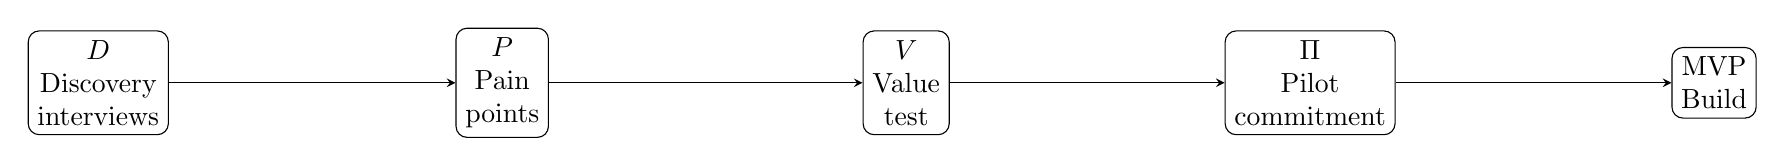
\begin{tikzpicture}[x=2.7cm,y=1.6cm,>=stealth]
\node[draw, rectangle, rounded corners, align=center] (d) at (0,0) {$D$\\Discovery\\interviews};
\node[draw, rectangle, rounded corners, align=center] (p) at (1.9,0) {$P$\\Pain\\points};
\node[draw, rectangle, rounded corners, align=center] (v) at (3.8,0) {$V$\\Value\\test};
\node[draw, rectangle, rounded corners, align=center] (pi) at (5.7,0) {$\Pi$\\Pilot\\commitment};
\node[draw, rectangle, rounded corners, align=center] (mvp) at (7.6,0) {$\mathrm{MVP}$\\Build};
\draw[->] (d) -- (p);
\draw[->] (p) -- (v);
\draw[->] (v) -- (pi);
\draw[->] (pi) -- (mvp);
\end{tikzpicture}
\caption{Transcript-derived schematic of the pre-build validation sequence described in the interview.}
\end{figure}

We may say this another way. The lecture insists that entrepreneurship begins as disciplined listening. We do not yet know what the product is, in a business sense, until we know how the prospective customer experiences the problem.

\section{When Is an Idea Worth Further Investment?}

\subsection{Question \& Answer}

The next question is the right one to ask after discovery. Suppose an idea now has a small team around it, and some money has begun to gather around it. At what point do we know that it is worth continuing? The lecture answers by tightening the criterion.

John's answer is that solving a serious problem is not enough. A problem may be large, genuine, and painful, and still not support a scalable business. What matters is whether the entrepreneur has figured out a way to get customers and repeat that process at scale. In our shorthand,
\begin{equation}
G \Leftarrow A_{\mathrm{cust}} \land S,
\qquad
G \not\Leftarrow \text{problem importance alone}.
\end{equation}
Here \(G\) means that the idea is good in the narrow operational sense of meriting further investment, \(A_{\mathrm{cust}}\) denotes a workable customer-acquisition mechanism, and \(S\) denotes a path to scale.

\begin{remark}
This equation should be read cautiously. It is a compact summary of a verbal criterion, not a necessary-and-sufficient theorem. The lecture's point is directional: the scale question is decisive in a way that mere importance is not.
\end{remark}

That is the conceptual pivot of the chapter. We are moved from the language of inspiration to the language of acquisition. A business idea becomes legible not when it sounds impressive, but when it can cross the gap from isolated value to repeatable customer capture.

\section{Perfectionism and the Discipline of Feedback}

\subsection{Question \& Answer}

Once the lecture has shifted us toward customer acquisition and scale, the next obstacle appears almost inevitably: perfectionism. What should the entrepreneur do if the product is never sent out because it is never judged good enough?

John's answer is psychologically sharp. Perfectionism is treated not as a badge of standards, but as a form of insecurity. The founder is afraid of hearing that the baby is ugly, and so the baby is never shown. In technical terms, perfectionism interrupts the feedback loop that makes improvement possible.

A faithful schematic of the lecture's logic is
\begin{equation}
\text{Prototype}_0
\xrightarrow{\text{client feedback}}
\text{Prototype}_1
\xrightarrow{\text{client feedback}}
\text{Prototype}_2
\rightarrow \cdots
\end{equation}
The lecture does not present this as formal notation, but it captures the procedural idea exactly. We begin with something imperfect yet differentiated, place it in front of the customer, and use the customer's response to reshape the next version.

There are several important elements here.
\begin{itemize}
\item The product need not be perfect.
\item The founder may admit openly that it is not perfect.
\item The customer is not merely a buyer, but also a shaper of fit.
\item Early exposure creates the possibility of course correction.
\end{itemize}

Thus the lecture treats imperfection not as a defect to be concealed, but as a condition under which learning becomes possible. This section belongs where it does because it answers the emotional resistance that follows naturally once the founder has accepted the need for customer validation.

\section{Failure, Fundraising, and the Signals That Matter}

Before the lecture answers the capital question, it pauses over failure. That pause is crucial. Adversity and setbacks are not presented as evidence that the journey has gone wrong; rather, they are presented as the journey's shaping force. The destination may include an exit or an IPO, but the lecture insists that the entrepreneur is formed by the obstacles met on the way there.

Only then does the lecture turn explicitly to fundraising. John's point is again subtractive: there is no magic number at which the founder suddenly becomes investment-worthy. What matters instead is a bundle of signals. We may summarize them, cautiously, as
\begin{equation}
R_{\mathrm{raise}} \Leftarrow U \land A_{\mathrm{rep}} \land \mathcal{P} \land (\Delta \mathrm{MRR} > 0).
\end{equation}
Here \(R_{\mathrm{raise}}\) denotes fundraising readiness, \(U\) denotes visible upside or potential, \(A_{\mathrm{rep}}\) denotes repeatable customer acquisition, \(\mathcal{P}\) denotes a credible plan, and \(\Delta \mathrm{MRR} > 0\) means that monthly recurring revenue is improving month to month. John also stresses that early product testing is cheaper now than it once was, and therefore the entrepreneur should test first, reinvest early revenue if possible, broaden traction, and only then take the business out for investment.

\paragraph{Worked example.}
Suppose we use a purely illustrative monthly recurring revenue update:
\begin{align}
\mathrm{MRR}_0 &= \$8{,}000, &
\mathrm{MRR}_1 &= \$10{,}500, \\
\Delta \mathrm{MRR} &= \mathrm{MRR}_1 - \mathrm{MRR}_0 = \$2{,}500 > 0.
\end{align}
This does \emph{not} prove that the company is investable. The lecture is explicit that there is no single threshold. But this is the direction of travel John wants to see: traction that is not merely anecdotal, but cumulative and increasingly legible.

The lecture's logic, then, is sequential. We do not raise money because the idea is emotionally compelling. We raise money because the business is beginning to show signs of repeatability.

\section{Scaling, Marketing, Exit, Advisors, and Haymaker}

The final movement of the lecture compresses several later-stage judgments, but they remain connected if we read them in order.

First comes scaling through delegation. John's rule is simple and practical:
\begin{equation}
\text{Outsource if } c_{\mathrm{task}} < r_{\mathrm{founder}}.
\end{equation}
Here \(c_{\mathrm{task}}\) is the outside cost of getting a task done and \(r_{\mathrm{founder}}\) is the founder's effective hourly value. If a permanent role is required, then the decision is no longer a casual outsourcing choice; it enters the forecast and the budget.

\paragraph{Worked example.}
Take a stylized case:
\begin{align}
r_{\mathrm{founder}} &= \$200/\text{hr}, &
c_{\mathrm{task}} &= \$45/\text{hr}, \\
c_{\mathrm{task}} < r_{\mathrm{founder}}
&\Longrightarrow \text{delegate the task.}
\end{align}
Again, the lecture does not claim that this rule solves everything. It ignores management overhead, strategic sensitivity, and quality variation. But it is exactly the sort of operating heuristic that appears once a founder begins to think in terms of leverage rather than merely effort.

Second comes the marketing split. The lecture distinguishes enterprise from consumer plays, not by abstract taxonomy, but by channel mix.

\begin{table}[h]
\centering
\begin{tabular}{|l|l|}
\hline
Business type & Dominant channels emphasized in the lecture \\
\hline
Enterprise & Email, direct outreach, possible cold calling, social mix \\
Consumer & Social-media-heavy acquisition \\
\hline
\end{tabular}
\caption{Transcript-derived marketing split.}
\end{table}

Third comes the exit question. The advice is pointedly unromantic: focus on the bottom line, keep building revenue, keep moving the needle efficiently, and let investors or acquirers notice what the company is already doing well. In compact form,
\begin{equation}
E_{\mathrm{exit}} \uparrow
\qquad \text{as} \qquad
\mathrm{Revenue} \uparrow \ \text{and operating efficiency improves}.
\end{equation}
This is not a valuation formula. It is a statement of posture. One does not optimize first for the story of selling; one optimizes first for performance that attracts institutional notice.

The mentor section fits naturally here. The lecture argues against the fantasy of one master advisor. The founder needs a circle: one person for motivation, others for sales, operations, and the subtler categories in which no single entrepreneur is expert. Running a business is presented as too nuanced for a single-source model of wisdom.

Finally, the lecture returns to Haymaker, and this return gives the chapter its concrete landing point. Haymaker is described as a marketplace for temporary office and meeting space: luxury homes, flex spaces, studios, and more traditional commercial real estate, all made available by the hour or day. The deeper business point is the pivot. A pre-pandemic coworking idea is re-read under pandemic conditions and redirected toward meeting space as companies reduce fixed real-estate footprints. We might summarize the model as
\begin{equation}
\text{distributed work patterns}
\longrightarrow
\text{reduced permanent footprint}
\longrightarrow
\text{demand for flexible meeting and office inventory}.
\end{equation}
Thus the lecture ends where it began: not with startup mythology, but with the disciplined reading of how demand changes in the world and how a company can reposition itself around that change.

\section{Summary}

The chapter begins with a noisy field of business advice and gradually extracts a sharper founder logic. We start with teaser questions, ambient stories of money and rejection, and then move into John Abraham's more disciplined account of startup building. The core lesson is ordered and cumulative: validate before building, test value with decision-makers, seek pilot commitments, do not confuse a serious problem with a scalable company, expose imperfect work to feedback, read adversity as formative rather than disqualifying, raise capital from traction, delegate by leverage, market differently depending on the buyer, and prepare for exit by building a business whose operating performance is already hard to ignore.

What makes the lecture strong is not that it offers a hidden formula. It is that it repeatedly removes false criteria and replaces them with operational ones. We are asked to trade inspiration for validation, secrecy for feedback, and vague ambition for disciplined movement in revenue, acquisition, and execution.